\chapter{Metodología}
A lo largo de este capitulo señalaremos la forma y con qué métodos llegaremos, con éxito, al objetivo de este proyecto
\section{Algoritmos de Minería de Datos}
A continuación se presentan las diferentes opciones utilizadas en las literaturas consultadas sobre \textit{Educational Data Mining(EDM)}\cite{EDMSurv} y una breve descripción de estos:
\begin{description}
  \item[Decision Tree Learning] \hfill \\
  Modelo de predicción basado en árboles de decisiones que entrega las clasificaciones de una forma clara y sencilla.
  \item[Hierarchical Clustering] \hfill \\
  Modelo de predicción basado en la búsqueda de \textit{clusters} con relaciones jerárquicas entre ellos.
  \item[Logistic Regression] \hfill \\
  Modelo probabilístico que busca clasificación en variables discretas. 
    \item[Linear/Multiple Regression] \hfill \\
  Modelo probabilístico que busca establecer una relación entre dos vectores. \newpage
  \item[K-means Clustering] \hfill \\
  Método de \textit{clustering} que consiste que busca particionar $n$ observaciones en $k$ \textit{clusters} utilizando por ejemplo la distancia promedio entre las observaciones para clasificar.
  \item[Naive Bayes] \hfill \\
  Clasificador estadístico que asume independencia en las variables para lograr clasificar las observaciones en diferentes categorías.
  \item[Support Vector Machine] \hfill \\
  Método que busca particionar las observaciones utilizando hiperplanos para lograr el \textit{clustering} de estos mismos.
  \item[Artificial Neural Networks] \hfill \\
  Método de predicción que asimila a la función biológica del cerebro, es decir, se compone de varios nodos interconectados que se asemejan a las neuronas para lograr clasificar información.
\end{description}
Los algoritmos señalados anteriormente están disponibles en diferentes  herramientas y/o lenguajes, pero se preferirán herramientas de carácter libre(sin costo) con la finalidad de que el proyecto tenga un costo cercano a cero. Un tema importante que sí considera costos son los recursos computacionales debido a la necesidad de escalamiento. Para esto, existe la posibilidad de utilizar de forma gratuita el laboratorio experimental de Cloud en la Universidad Adolfo Ibáñez. De no ser posible, se preferirá el uso de herramientas como \textit{Amazon AWS} o \textit{Microsoft Azure} que usan un sistema de costeo por horas de procesamiento. Actualmente sería difícil estimar el costo de esto de forma precisa. Una cifra estimativa son 100 horas destinadas al desarrollo del proyecto. Utilizando \textit{Microsoft Azure} tendría un costo aproximado de 150 dólares\footnote{Consultado en el mes de Junio del año 2015 desde \url{http://azure.microsoft.com/en-us/pricing/details/machine-learning/}}.

\section{Herramientas de Minería de Datos}
A continuación se presentará el \textit{software} que será utilizado para lograr los objetivos del trabajo.
\subsection{R-project\cite{rproject}}
R es un lenguaje de programación que se utiliza ampliamente en el área científica para estudios estadísticos. Es relativamente sencillo de utilizar, sin embargo no es la mejor opción cuando se requiere manejar grandes volúmenes de datos.
\subsection{Python Anaconda Package\cite{python}}
Python es un lenguaje de programación multi-paradigma, es decir, soporta orientación tanto a objetos como programación imperativa y, en menor medida, programación funcional.
Lo bueno de este lenguaje de programación es que tiene mucho potencial, y en consecuencia, facilita el pre-procesamiento de los datos.
Se utilizará un paquete libre llamado Anaconda que recopila los módulos necesarios para trabajar con estadística y \textit{Machine Learning}.
\subsection{WEKA\cite{weka}}
WEKA es una plataforma de software para el aprendizaje automático y la minería de datos escrito en Java.
El plus de este software es la interfaz gráfica que presenta y le da facilidad de uso. Además, al igual que Python, WEKA es totalmente gratuito.
\subsection{Apache Hadoop\cite{hadoop}}
Al hablar de Hadoop señalamos el stack de software que desarrolló Apache para trabajar con procesamiento paralelo y mucha información. Normalmente el stack consiste en HDFS, YARN, Hive, Pig, Spark, HBase, MapReduce, Kafka y Mahout.
\section{Metodología de Minería de Datos}
Para lograr nuestro objetivo utilizaremos como metodología CRISP-DM\footnote{\url{Sobre CRISP-DM: http://www.the-modeling-agency.com/crisp-dm.pdf}} y SEMMA\footnote{\url{Sobre SEMMA: http://webdocs.cs.ualberta.ca/~zaiane/courses/cmput690/work/group4/sas.pdf}} de referencia.La razón del por qué utilizamos estas metodologías de referencia es por que son las más reconocidas y utilizadas en el mundo científico\cite{crispol,crispol2,crispol3}. En la Figura~\ref{fig:metdat} se presenta la metodología adoptada.
\begin{description}
  \item[Entendimiento de la información] \hfill \\
  Se debe tener una comprensión de la información para poder manipular la información y entender lo que se hace
  \item[Selección de la información valiosa] \hfill \\
  Es necesario seleccionar la información justa y necesaria, pues entre más datos entra al modelo, puede generar ruido en la salida del modelo.
  \item[Pre-procesamiento de la información valiosa] \hfill \\
  No se puede asumir que la calidad de la información es óptima, por tanto, se debe hacer una revisión de la información seleccionada en busca de datos anómalos y reparación de estos. Todo esto nuevamente  es para evitar ruido en la salida del modelo y resultados no deseados.
  \item[Creación de modelos predictivos] \hfill \\
  En esta parte se aplica el modelo y se procede a la predicción de la deserción escolar.
  \item[Interpretación de los resultados] \hfill \\
  Finalmente se prosigue con la interpretación de los resultados y la comparación frente a la teoría estudiada y resultados empíricos anteriores.
\end{description}

\begin{figure}[H]
  \centering
    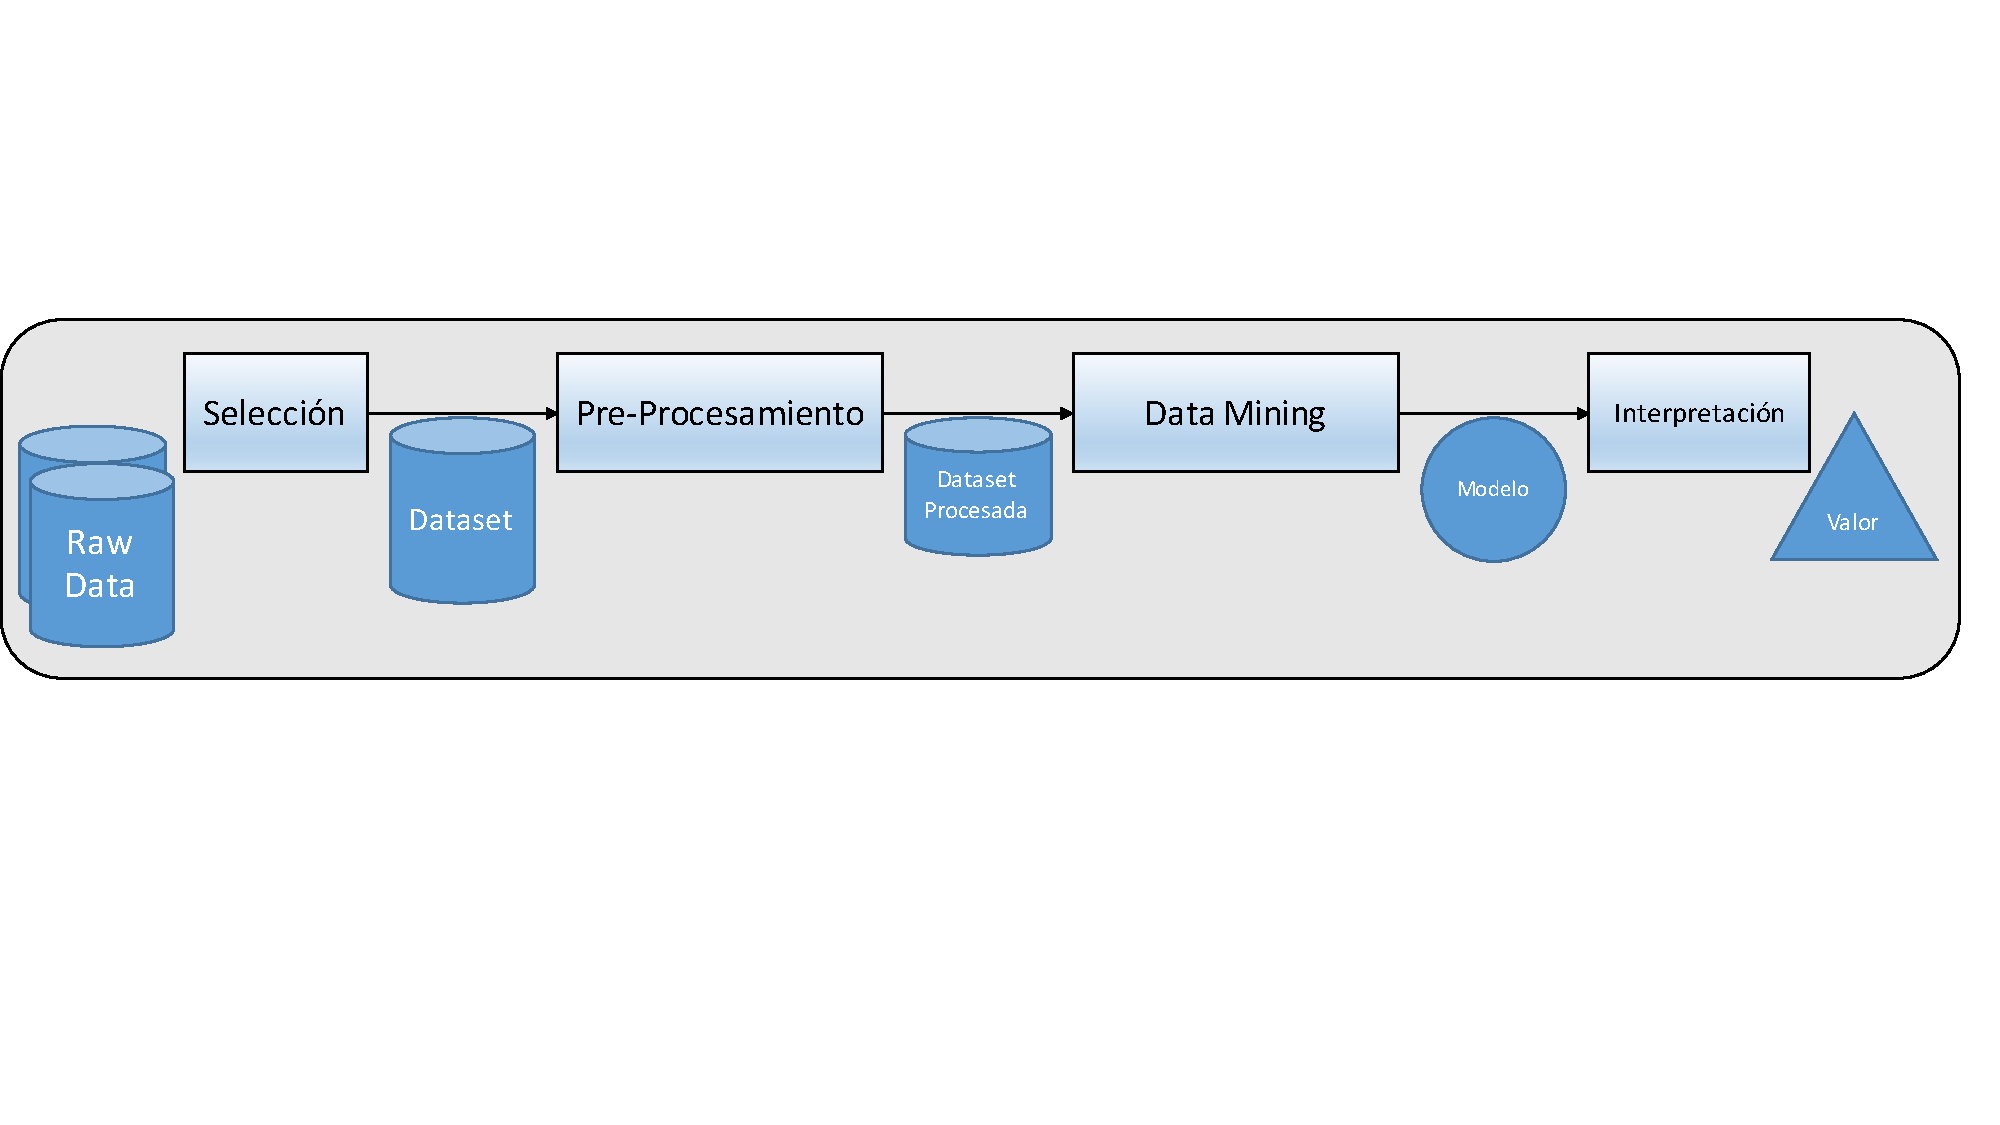
\includegraphics[width=0.7\textwidth]{Figuras/Metodologia}
      \caption{Metodología de Minería de Datos para el presente proyecto}
    \label{fig:metdat}
\end{figure}
\section{Conclusiones}
Finalmente a modo de resumen de la metodología y marco de trabajo adoptado se optará por probar la mayor cantidad de algoritmos de minería de datos y escoger el que entregue mejores resultados al menor costo. Lo mismo con las herramientas; Python será útil para el pre-procesamiento y exploración, pero R apoyará en la creación de un modelo predictivo y hacer el análisis comparativo. Finalmente se analizará la necesidad de escalamiento y en base a los requerimientos puntuales se escogerá un \textit{stack} de \textit{Hadoop} que satisfaga los requerimientos del proyecto pensando en la minimización de costos.